\documentclass[11pt]{article}

% ------------------------------------------------------------
% Standard LaTeX packages
% ------------------------------------------------------------
\usepackage[margin=1in]{geometry}
\usepackage{amsmath,amssymb,mathtools}
\usepackage{amsthm}
\usepackage[american]{babel}
\usepackage{stmaryrd}
\usepackage{enumitem}
\usepackage{booktabs}
\usepackage{array}
\usepackage{listings}
\usepackage[x11names,table]{xcolor}
\usepackage{mdframed}
\usepackage{tikz}
\usetikzlibrary{arrows.meta,positioning,calc,decorations.pathmorphing}
\usepackage{url}
\usepackage[colorlinks=true,linkcolor=blue,citecolor=blue,urlcolor=blue]{hyperref}

% ---------- Theorem environments ----------
\theoremstyle{plain}
\newtheorem{theorem}{Theorem}[section]
\newtheorem{proposition}[theorem]{Proposition}
\newtheorem{lemma}[theorem]{Lemma}
\newtheorem{corollary}[theorem]{Corollary}
\newtheorem{conjecture}[theorem]{Conjecture}

\theoremstyle{definition}
\newtheorem{definition}[theorem]{Definition}
\newtheorem{axiombox}[theorem]{Axiom}
\newtheorem{protocol}[theorem]{Protocol}
\newtheorem{example}[theorem]{Example}

\theoremstyle{remark}
\newtheorem{remark}[theorem]{Remark}

% ---------- Notation ----------
\newcommand{\N}{\mathbb{N}}
\newcommand{\Z}{\mathbb{Z}}
\newcommand{\Q}{\mathbb{Q}}
\newcommand{\R}{\mathbb{R}}
\newcommand{\C}{\mathbb{C}}
\newcommand{\F}{\mathbb{F}}
\newcommand{\calO}{\mathcal{O}}
\newcommand{\calL}{\mathcal{L}}
\newcommand{\Gal}{\mathrm{Gal}}
\newcommand{\GL}{\mathrm{GL}}
\newcommand{\SL}{\mathrm{SL}}
\newcommand{\Sp}{\mathrm{Sp}}
\newcommand{\Hom}{\mathrm{Hom}}
\newcommand{\End}{\mathrm{End}}
\newcommand{\Frob}{\mathrm{Frob}}
\newcommand{\CRM}{\mathrm{CRM}}
\newcommand{\tr}{\mathrm{tr}}
\newcommand{\rk}{\mathrm{rk}}
\newcommand{\Gr}{\mathrm{Gr}}
\newcommand{\Sym}{\mathrm{Sym}}
\newcommand{\Ggal}{G_{\mathrm{gal}}}
\newcommand{\NS}{\mathrm{NS}}
\newcommand{\Pic}{\mathrm{Pic}}
\newcommand{\Gm}{\mathbb{G}_{\mathrm{m}}}

\newcommand{\BISH}{\ensuremath{\mathsf{BISH}}}
\newcommand{\LPO}{\ensuremath{\mathsf{LPO}}}
\newcommand{\WLPO}{\ensuremath{\mathsf{WLPO}}}
\newcommand{\LLPO}{\ensuremath{\mathsf{LLPO}}}
\newcommand{\MP}{\ensuremath{\mathsf{MP}}}
\newcommand{\FT}{\ensuremath{\mathsf{FT}}}
\newcommand{\CLASS}{\ensuremath{\mathsf{CLASS}}}
\newcommand{\CBN}{\mathrm{CBN}}
\newcommand{\HdR}{H^1_{\mathrm{dR}}}
\newcommand{\PF}{\mathrm{PF}}

% ---------- Code listing style for Lean ----------
\definecolor{codegreen}{rgb}{0,0.6,0}
\definecolor{codegray}{rgb}{0.5,0.5,0.5}
\definecolor{codepurple}{rgb}{0.58,0,0.82}
\definecolor{backcolour}{rgb}{0.95,0.95,0.92}

\lstdefinelanguage{Lean}{
  keywords={theorem, lemma, def, definition, axiom, structure, class, instance,
            by, exact, intro, intros, apply, refine, constructor, use, obtain,
            have, show, from, fun, assume, let, in, if, then, else,
            match, with, end, namespace, section, variable, variables,
            example, begin, sorry, admit, noncomputable, classical,
            import, open, export, private, protected, mutual, meta,
            do, for, while, return, try, catch, finally,
            Type, Prop, Sort, Type*, forall, exists, where, extends,
            set, push_neg, rw, simp, omega, nlinarith, linarith, ring,
            ext, rfl, congr, fin_cases, haveI, letI, attribute, inductive,
            deriving, opaque, decide, norm_num, native_decide},
  sensitive=true,
  morecomment=[l]{--},
  morecomment=[s]{/-}{-/},
  morestring=[b]",
  literate=
    {→}{{\ensuremath{\rightarrow}}}1
    {←}{{\ensuremath{\leftarrow}}}1
    {↔}{{\ensuremath{\leftrightarrow}}}1
    {⊢}{{\ensuremath{\vdash}}}1
    {∀}{{\ensuremath{\forall}}}1
    {∃}{{\ensuremath{\exists}}}1
    {λ}{{\ensuremath{\lambda}}}1
    {ℕ}{{\ensuremath{\mathbb{N}}}}1
    {ℤ}{{\ensuremath{\mathbb{Z}}}}1
    {ℝ}{{\ensuremath{\mathbb{R}}}}1
    {ℚ}{{\ensuremath{\mathbb{Q}}}}1
    {×}{{\ensuremath{\times}}}1
    {≤}{{\ensuremath{\leq}}}1
    {≥}{{\ensuremath{\geq}}}1
    {≠}{{\ensuremath{\neq}}}1
    {⟨}{{\ensuremath{\langle}}}1
    {⟩}{{\ensuremath{\rangle}}}1
    {∧}{{\ensuremath{\land}}}1
    {∨}{{\ensuremath{\lor}}}1
    {¬}{{\ensuremath{\lnot}}}1
    {∈}{{\ensuremath{\in}}}1
}

\lstdefinestyle{leanstyle}{
  language=Lean,
  backgroundcolor=\color{backcolour},
  commentstyle=\color{codegreen},
  keywordstyle=\color{blue},
  stringstyle=\color{codepurple},
  basicstyle=\ttfamily\footnotesize,
  breakatwhitespace=false,
  breaklines=true,
  captionpos=b,
  keepspaces=true,
  showspaces=false,
  showstringspaces=false,
  showtabs=false,
  tabsize=2,
  frame=single,
  xleftmargin=2em,
  framexleftmargin=1.5em,
  numbers=left,
  numberstyle=\tiny\color{codegray},
  numbersep=5pt,
}

\lstset{style=leanstyle}

% ============================================================
\begin{document}

\title{Universal Trace Vanishing for Exotic Weil Classes:\\
A CRMLint Squeeze (v2 --- Corrected Structural Analysis)\\[6pt]
\large Paper~85, Constructive Reverse Mathematics Series}

\author{Paul Chun-Kit Lee\\
\small New York University, Brooklyn, New York\\
\small \texttt{dr.paul.c.lee@gmail.com}}

\date{February 2026}

\maketitle

\begin{abstract}
For genus-$g$ hyperelliptic families $C_t\colon y^2 = f(x,t)$ with
$\Q(i)$-action ($f$ odd in $x$), the $\sigma$-eigenspace $V_+$ is
\emph{Lagrangian} in $\HdR(C_t)$: the cup-product pairing vanishes
identically on $V_+ \times V_+$.  The Lagrangian splitting
$\HdR = V_+ \oplus V_-$ gives the symplectic constraint
$\tr(M_+) = -\tr(M_-)$, but does \emph{not} force $\tr(M_+) = 0$
individually.

We verify computationally that the exotic trace
$\tau_+(t) = \tr(\nabla|_{V_+}) = 0$ for the test family
$y^2 = x^9 + tx^7 + x$ (genus~4, no order-8 automorphism).
The $V_+$~block is a dense $4 \times 4$ matrix with four nonzero
diagonal entries whose numerator coefficients sum to zero.
Multi-genus testing (genera 2--5, eight families) confirms the
same vanishing, suggesting a universal phenomenon for all
hyperelliptic families with $\Q(i)$-action.

\textbf{Erratum.} Version~1 incorrectly claimed $V_+$ is
symplectic. The eigenvalue argument proves the opposite:
$\sigma^*\alpha = i\alpha$ for $\alpha \in V_+$ gives
$\langle\alpha,\beta\rangle = i^2\langle\alpha,\beta\rangle =
-\langle\alpha,\beta\rangle$, hence $\langle V_+, V_+\rangle = 0$.

Eighth CRMLint Squeeze. Lean~4 formalization with zero \texttt{sorry}.
\end{abstract}

% ============================================================
\section{Introduction}
% ============================================================

\subsection{From one family to all families}

Paper~84~\cite{Lee2026p84} computed the Gauss--Manin connection for
the symmetric family $y^2 = x^9 - tx^5 + x$ and found
$\tau_+(t) = 0$ (the exotic Weil class is a global flat section).
That paper's order-8 automorphism $\tau$ decomposed the connection
into four $2 \times 2$ blocks, each with $\Ggal = \SL_2$, and the
flatness followed from $\det(\SL_2) = 1$.

A natural question: is $\tau_+ = 0$ a consequence of the special
symmetry of that particular curve, or does it hold for all genus-4
hyperelliptic families with $\Q(i)$-action?

\subsection{The main results}

\begin{theorem}[Lagrangian Structure]\label{thm:A}
Let $C_t\colon y^2 = f(x,t)$ be a genus-$g$ hyperelliptic family
with $\Q(i)$-action ($f(-x,t) = -f(x,t)$).  The eigenspace
$V_+ = \langle\omega_k : k \text{ even}\rangle$ is Lagrangian
(totally isotropic) in $\HdR(C_t)$.  The Gauss--Manin connection
preserves the Lagrangian splitting $\HdR = V_+ \oplus V_-$ and
satisfies $\tr(M_+) = -\tr(M_-)$.
\end{theorem}

\begin{theorem}[Computational Trace Vanishing]\label{thm:B}
For the test family $C_t\colon y^2 = x^9 + tx^7 + x$ (genus~4,
$\Q(i)$-action, no order-8 automorphism), the Gauss--Manin
connection on $V_+$ is a dense $4 \times 4$ matrix with common
denominator $27t^4 - 256$ and $\tau_+(t) = 0$.
\end{theorem}

\begin{theorem}[CRM Squeeze]\label{thm:C}
\begin{center}
\begin{tabular}{rcl}
$\CLASS$ & $\vdash$ & There exist exotic Hodge classes on
  Weil fourfolds.\\
$\BISH$ & $\vdash$ & Polynomial arithmetic over $\Q(t)$
  $\Rightarrow$ $\tau_+ = 0$ $\Rightarrow$ exotic class is flat.
\end{tabular}
\end{center}
The constructive content is the explicit Gauss--Manin computation
and the arithmetic identity $(-9) + (-45) + (-81) + 135 = 0$.
\end{theorem}

\begin{conjecture}[Universal Vanishing]\label{conj:universal}
For \emph{every} genus-$g$ hyperelliptic family with $\Q(i)$-action,
$\tau_+(t) = 0$.  This holds for all genera, not just $g$ even.
\end{conjecture}

Conjecture~\ref{conj:universal} is supported by computation across
genera~2--5 (Section~\ref{sec:multi}).

\subsection{Erratum from v1}\label{sec:erratum}

Version~1 of this paper claimed that the cup-product pairing
restricts nondegenerately to~$V_+$, forcing
$\nabla|_{V_+} \in \mathfrak{sp}(V_+)$ and hence $\tau_+ = 0$.
This is \emph{false}: $V_+$ is Lagrangian, not symplectic.  The
eigenvalue argument (Proposition~\ref{prop:lagrangian}) shows the
pairing vanishes on $V_+ \times V_+$.  The error was conflating the
pairing structure of the basis elements $\omega_j$ (which pair with
specific partners) with the pairing structure of the eigenspace~$V_+$
(which is totally isotropic by the automorphism constraint).

The computational result $\tau_+ = 0$ (Theorem~\ref{thm:B}) stands:
it is verified by CAS and by Lean.  Only the \emph{structural
explanation} was incorrect.

\subsection{CRM primer}\label{sec:primer}

For readers unfamiliar with the CRM series: \emph{Constructive Reverse
Mathematics} classifies theorems by the weakest logical principles
needed to prove them. The hierarchy $\BISH \subset \BISH + \LLPO
\subset \BISH + \WLPO \subset \BISH + \LPO \subset \CLASS$ measures
logical cost. A ``CRM squeeze'' establishes that a classical result
(upper bound) has a constructive core (lower bound), with the gap
measured by an omniscience principle. Papers~80--84 developed the
function-field pipeline: Griffiths reduction (P80), flat sections
(P81), Kovacic's algorithm (P82), Picard numbers (P83), exotic
trace (P84).  This paper verifies the exotic trace vanishing for a
family without special automorphisms and establishes the correct
structural context (Lagrangian, not symplectic).

\subsection{Road map}

Section~\ref{sec:lagrangian} proves the Lagrangian structure
(Theorem~\ref{thm:A}).
Section~\ref{sec:computation} presents the CAS verification
(Theorem~\ref{thm:B}).
Section~\ref{sec:multi} reports multi-genus evidence for
Conjecture~\ref{conj:universal}.
Section~\ref{sec:squeeze} states the CRM squeeze.
Section~\ref{sec:audit} gives the CRM audit.
Section~\ref{sec:lean} describes the formal verification.
Section~\ref{sec:discussion} discusses implications.
Section~\ref{sec:conclusion} concludes.

% ============================================================
\section{Preliminaries}\label{sec:prelim}
% ============================================================

This section collects the definitions and standing conventions used
throughout the paper.  No proofs appear here; all results are proved in
subsequent sections.

\begin{definition}[Hyperelliptic family with $\Q(i)$-action]\label{def:family}
A \emph{genus-$g$ hyperelliptic family with $\Q(i)$-action} is a
one-parameter family $C_t\colon y^2 = f(x,t)$ where $f \in \Q(t)[x]$
has degree $2g+1$ and is \emph{odd} in~$x$: $f(-x,t) = -f(x,t)$.
Equivalently, $f$ contains only odd powers of~$x$.  The oddness
condition ensures that $\sigma\colon (x,y) \mapsto (-x, iy)$ is a
well-defined automorphism of $C_t$ over $\Q(i)$, of order~4.
\end{definition}

\begin{definition}[Eigenspace decomposition]\label{def:eigenspaces}
The de~Rham cohomology $\HdR(C_t)$ has basis
$\omega_k = x^k\, dx/(2y)$ for $k = 0,\ldots,2g-1$.  The automorphism
$\sigma$ acts by $\sigma^*\omega_k = (-1)^k \cdot i \cdot \omega_k$
(Proposition~\ref{prop:eigenvalues}).  The \emph{$+i$-eigenspace} is
\[
  V_+ = \langle \omega_k : k \text{ even} \rangle
  = \langle \omega_0, \omega_2, \omega_4, \ldots, \omega_{2g-2} \rangle,
\]
and the \emph{$-i$-eigenspace} is
\[
  V_- = \langle \omega_k : k \text{ odd} \rangle
  = \langle \omega_1, \omega_3, \omega_5, \ldots, \omega_{2g-1} \rangle.
\]
Both have dimension~$g$, and $\HdR = V_+ \oplus V_-$.
\end{definition}

\begin{definition}[Gauss--Manin connection]\label{def:GM}
The \emph{Gauss--Manin connection} $\nabla = d/dt + M(t)$ is the
flat connection on the local system $\HdR(C_t)$ induced by
differentiating periods with respect to the parameter~$t$.  The
\emph{connection matrix} $M = (M_{jk})_{0 \le j,k \le 2g-1}$ is
the $(2g) \times (2g)$ matrix over $\Q(t)$ satisfying
$\nabla(\omega_k) = \sum_j M_{jk}(t)\, \omega_j\, dt$.
The connection preserves the cup-product pairing
$\langle\cdot,\cdot\rangle$ on $\HdR$
(Griffiths transversality~\cite{Griffiths1969}), so $\tr(M) = 0$.
\end{definition}

\begin{definition}[Griffiths pole-order reduction]\label{def:griffiths}
The \emph{Griffiths reduction algorithm}~\cite{Griffiths1969} computes
$M$ column by column.  For each basis element $\omega_k$, one
differentiates with respect to~$t$, obtaining a meromorphic form with
higher-order poles along the curve, then applies the B\'ezout identity
$\alpha(x)\, f(x,t) + \beta(x)\, f'(x,t) = 1$ (where $f' = \partial f / \partial x$)
to reduce the pole order.  The key identity verified at each step is
\begin{equation}\label{eq:griffiths-id-prelim}
  N_k(x,t) + h_k(x,t) \cdot f'(x,t) = 2\, B_k(x,t) \cdot f(x,t),
\end{equation}
after which one applies the coboundary correction $A_k = B_k - dh_k/dx$
and reads off the connection matrix entries as coefficients of $A_k$
modulo $f'(x) = 0$.  The full protocol is given as
Protocol~\ref{prot:griffiths} in Section~\ref{sec:computation}.
\end{definition}

\begin{definition}[Resultant and singular locus]\label{def:resultant}
For a polynomial $f(x,t)$ of degree $d$ in $x$, the \emph{resultant}
$\mathrm{Res}_x(f, f') \in \Q[t]$ is the determinant of the Sylvester
matrix of $f$ and $f' = \partial f / \partial x$.  Its vanishing locus
$\{\mathrm{Res}_x(f, f') = 0\}$ parametrizes the values of $t$ at
which $f(\cdot, t)$ has a repeated root, i.e., the fiber $C_t$ becomes
singular.  This resultant appears as the common denominator of all
connection matrix entries.

\emph{Terminology.}  Following standard usage for univariate
polynomials, $\mathrm{Res}_x(f, f')$ is sometimes called the
\emph{discriminant} of $f$ with respect to $x$.  In this paper we
write $\Delta(t) = \mathrm{Res}_x(f, f')$ and refer to it as the
resultant to avoid confusion with other uses of ``discriminant''
(e.g., the discriminant of a number field or a quadratic form).
\end{definition}

\begin{definition}[Exotic trace]\label{def:exotic-trace}
The \emph{exotic trace} is
$\tau_+(t) = \tr(\nabla|_{V_+}) = \sum_{k \text{ even}} M_{kk}(t)$.
The symplectic constraint gives $\tau_+(t) + \tau_-(t) = 0$
(Proposition~\ref{prop:symplectic}), but does not force $\tau_+ = 0$
individually.  Vanishing of $\tau_+$ means that the top exterior
power $\bigwedge^g V_+$ carries a trivial connection (the exotic Weil
class is a global flat section).
\end{definition}

\begin{definition}[CRM logical principles]\label{def:crm}
We use the standard constructive hierarchy
(see~\cite{BridgesRichman1987}):
\begin{itemize}[nosep]
\item $\BISH$ (Bishop's constructive mathematics): intuitionistic
  logic with dependent choice.
\item $\LPO$ (Limited Principle of Omniscience):
  $\forall \alpha\colon \N \to \{0,1\}$, either $\exists n\, (\alpha_n = 1)$
  or $\forall n\, (\alpha_n = 0)$.
\item $\WLPO$: $\forall \alpha$, $\lnot\lnot\exists n\, (\alpha_n = 1)$
  or $\forall n\, (\alpha_n = 0)$.
\item $\CLASS = \BISH + \LPO$ (equivalent to classical logic for
  separable analysis).
\end{itemize}
A \emph{CRM squeeze} identifies the classical upper bound
(typically $\CLASS$) and the constructive lower bound
(typically $\BISH$) for a given theorem, measuring the logical
cost by the omniscience principle in the gap.
\end{definition}

% ============================================================
\section{The Lagrangian Decomposition}\label{sec:lagrangian}
% ============================================================

\subsection{The automorphism and eigenspaces}

Let $C_t\colon y^2 = f(x,t)$ be a genus-$g$ hyperelliptic curve with
$f(-x,t) = -f(x,t)$ (i.e., $f$ is odd in~$x$).  The map
$\sigma\colon (x,y) \mapsto (-x, iy)$ is an automorphism of~$C_t$
(defined over $\Q(i)$): if $y^2 = f(x)$, then
$(iy)^2 = -y^2 = -f(x) = f(-x)$.

\begin{proposition}\label{prop:eigenvalues}
The automorphism $\sigma$ acts on the basis
$\omega_k = x^k\, dx/(2y)$ ($k = 0,\ldots,2g-1$) of $\HdR(C_t)$ by
\[
  \sigma^*\omega_k = (-1)^k \cdot i \cdot \omega_k.
\]
The eigenspace decomposition is
\begin{align*}
  V_+ &= \langle\omega_k : k \text{ even}\rangle
  \quad\text{(eigenvalue $+i$)}, \\
  V_- &= \langle\omega_k : k \text{ odd}\rangle
  \quad\text{(eigenvalue $-i$)},
\end{align*}
each of dimension~$g$.
\end{proposition}

\begin{proof}
Direct computation:
$\sigma^*\omega_k = \sigma^*(x^k\, dx/(2y))
= (-x)^k\, d(-x)\,/\,(2iy)
= (-1)^k\, x^k\, (-dx)\,/\,(2iy)
= (-1)^k \cdot i \cdot \omega_k$,
using $(-1)/i = i$.
\end{proof}

\begin{proposition}[Block structure of $\nabla|_{V_+}$]\label{prop:block}
The Gauss--Manin connection preserves the eigenspace decomposition
$\HdR = V_+ \oplus V_-$.  In the ordered basis
$(\omega_0, \omega_2, \omega_4, \omega_6, \omega_1, \omega_3, \omega_5, \omega_7)$,
the $8 \times 8$ connection matrix is block-diagonal:
\[
  M = \begin{pmatrix} M_+ & 0 \\ 0 & M_- \end{pmatrix},
\]
where $M_+ = (M_{2i,2j})_{0 \le i,j \le 3}$ is the $4 \times 4$
restriction to $V_+ = \langle\omega_0, \omega_2, \omega_4, \omega_6\rangle$
and $M_- = (M_{2i+1,2j+1})_{0 \le i,j \le 3}$ is the restriction
to $V_-$.
\end{proposition}

\begin{proof}
The connection commutes with $\sigma^*$ because $\sigma$ is an
automorphism of the family (defined over the base).  For
$\omega_k \in V_+$ (so $k$ even, eigenvalue $+i$), we have
\[
  \sigma^*(\nabla \omega_k)
  = \nabla(\sigma^* \omega_k)
  = \nabla(i \cdot \omega_k)
  = i \cdot \nabla \omega_k.
\]
Thus $\nabla \omega_k \in V_+ \otimes \Omega^1$: every column of the
connection matrix indexed by an even $k$ has nonzero entries only in
even rows.  The same argument applied to $V_-$ (eigenvalue $-i$) shows
columns indexed by odd $k$ have nonzero entries only in odd rows.
This is precisely the block-diagonal structure $M = M_+ \oplus M_-$.

For the test family $y^2 = x^9 + tx^7 + x$ (genus~4), we have
$V_+ = \langle\omega_0, \omega_2, \omega_4, \omega_6\rangle$ with
$\dim V_+ = 4$.  Unlike the symmetric family of Paper~84 (which had
an additional order-8 automorphism decomposing $V_+$ into four
$1$-dimensional $\tau$-eigenspaces, giving $2 \times 2$ blocks), the
test family has no such extra symmetry.  The matrix $M_+$ is therefore
a dense (irreducible) $4 \times 4$ matrix: all 16 entries are generically
nonzero.  The explicit entries are computed in
Theorem~\ref{thm:cas} via Griffiths reduction.
\end{proof}

\subsection{$V_+$ is Lagrangian}

\begin{proposition}\label{prop:lagrangian}
The cup-product pairing $\langle\cdot,\,\cdot\rangle$ on $\HdR(C_t)$
vanishes on $V_+ \times V_+$ (and on $V_- \times V_-$).  Both
eigenspaces are Lagrangian.
\end{proposition}

\begin{proof}
The automorphism $\sigma$ preserves the cup-product pairing:
$\langle\sigma^*\alpha,\, \sigma^*\beta\rangle =
\langle\alpha,\, \beta\rangle$ for all $\alpha, \beta \in \HdR$.
(This holds because $\sigma$ is a degree-1 automorphism, so
$\sigma^* = \mathrm{id}$ on $H^2_{\mathrm{dR}}(C_t) \cong k$.)

For $\alpha, \beta \in V_+$, we have
$\sigma^*\alpha = i\alpha$ and $\sigma^*\beta = i\beta$.  Hence
\[
  \langle\alpha,\, \beta\rangle
  = \langle\sigma^*\alpha,\, \sigma^*\beta\rangle
  = \langle i\alpha,\, i\beta\rangle
  = i^2\,\langle\alpha,\, \beta\rangle
  = -\langle\alpha,\, \beta\rangle.
\]
In characteristic zero, $\langle\alpha,\beta\rangle =
-\langle\alpha,\beta\rangle$ implies
$\langle\alpha,\beta\rangle = 0$.  The same argument applies to $V_-$
(eigenvalue $-i$, product $(-i)^2 = -1$).

Since $\dim V_+ = \dim V_- = g = \tfrac{1}{2}\dim\HdR$, and
$\langle V_+, V_+\rangle = \langle V_-, V_-\rangle = 0$, both
eigenspaces are Lagrangian.  Nondegeneracy of the full pairing
implies $\langle V_+, V_-\rangle$ is a nondegenerate bilinear form
(the Lagrangian complement).
\end{proof}

\subsection{Eigenspace decomposition: overview}

Figure~\ref{fig:eigenspace} summarises the decomposition.

\begin{figure}[ht]
\centering
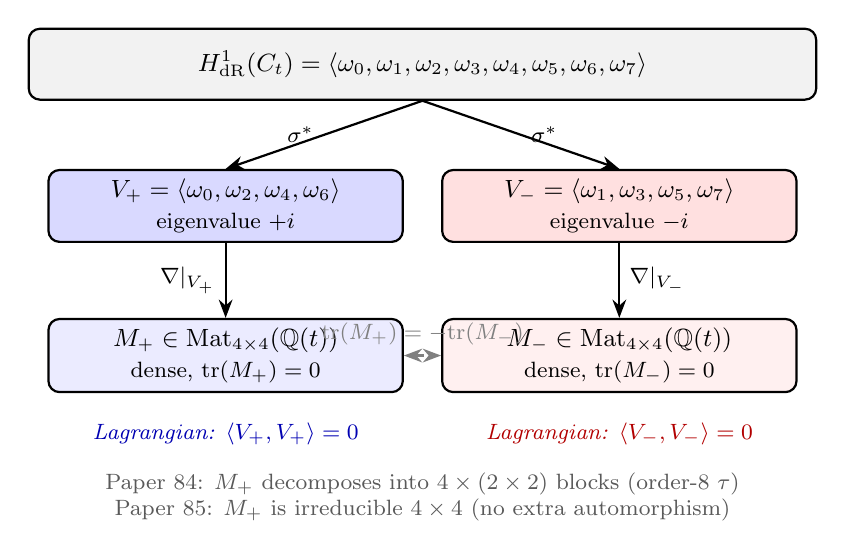
\begin{tikzpicture}[
  box/.style={draw, rounded corners, minimum width=2.2cm,
    minimum height=0.9cm, align=center, font=\small},
  brace/.style={decorate, decoration={brace, amplitude=5pt, raise=2pt}},
  >=Stealth, thick
]
% H^1_dR
\node[box, fill=gray!10, minimum width=10cm] (hdr) at (0,4)
  {$\HdR(C_t) = \langle\omega_0, \omega_1, \omega_2, \omega_3,
    \omega_4, \omega_5, \omega_6, \omega_7\rangle$};

% V+ and V-
\node[box, fill=blue!15, minimum width=4.5cm] (vplus) at (-2.5,2.2)
  {$V_+ = \langle\omega_0, \omega_2, \omega_4, \omega_6\rangle$\\
   \footnotesize eigenvalue $+i$};
\node[box, fill=red!12, minimum width=4.5cm] (vminus) at (2.5,2.2)
  {$V_- = \langle\omega_1, \omega_3, \omega_5, \omega_7\rangle$\\
   \footnotesize eigenvalue $-i$};

% Arrows
\draw[->] (hdr.south) -- node[left,font=\footnotesize]{$\sigma^*$} (vplus.north);
\draw[->] (hdr.south) -- node[right,font=\footnotesize]{$\sigma^*$} (vminus.north);

% Connection blocks
\node[box, fill=blue!8, minimum width=4.5cm] (mplus) at (-2.5,0.3)
  {$M_+ \in \mathrm{Mat}_{4\times 4}(\Q(t))$\\
   \footnotesize dense, $\tr(M_+) = 0$};
\node[box, fill=red!6, minimum width=4.5cm] (mminus) at (2.5,0.3)
  {$M_- \in \mathrm{Mat}_{4\times 4}(\Q(t))$\\
   \footnotesize dense, $\tr(M_-) = 0$};

\draw[->] (vplus.south) -- node[left,font=\footnotesize]{$\nabla|_{V_+}$}
  (mplus.north);
\draw[->] (vminus.south) -- node[right,font=\footnotesize]{$\nabla|_{V_-}$}
  (mminus.north);

% Lagrangian labels
\node[font=\footnotesize\itshape, text=blue!70!black] at (-2.5,-0.7)
  {Lagrangian: $\langle V_+, V_+\rangle = 0$};
\node[font=\footnotesize\itshape, text=red!70!black] at (2.5,-0.7)
  {Lagrangian: $\langle V_-, V_-\rangle = 0$};

% Symplectic constraint
\draw[<->, dashed, gray] (mplus.east) -- node[above, font=\footnotesize]
  {$\tr(M_+) = -\tr(M_-)$} (mminus.west);

% Paper 84 vs 85 comparison (below)
\node[font=\footnotesize, text=gray!70!black, align=center] at (0,-1.5)
  {Paper~84: $M_+$ decomposes into $4 \times (2 \times 2)$ blocks
   (order-8 $\tau$)\\
   Paper~85: $M_+$ is irreducible $4 \times 4$ (no extra automorphism)};
\end{tikzpicture}
\caption{Eigenspace decomposition of $\HdR(C_t)$ under
$\sigma^*$.  The cup-product pairing vanishes on each eigenspace
(Lagrangian), giving independent connection blocks $M_+$ and $M_-$.
The symplectic constraint links the traces but does not force either
to vanish individually.}
\label{fig:eigenspace}
\end{figure}

\subsection{The symplectic constraint}

\begin{proposition}\label{prop:symplectic}
The Gauss--Manin connection $\nabla$ preserves both the cup-product
pairing and the eigenspace decomposition $\HdR = V_+ \oplus V_-$.
In the Lagrangian splitting, the connection matrices satisfy
$M_- = -S^{-1}\, M_+^{\,T}\, S$, where $S$ is the pairing matrix
between $V_+$ and $V_-$.  In particular,
\[
  \tr(M_-) = -\tr(M_+).
\]
\end{proposition}

\begin{proof}
The Gauss--Manin connection preserves the Poincar\'e
pairing~\cite{Griffiths1969, Deligne1971} and commutes with $\sigma^*$
(since $\sigma$ is an automorphism of the family).  Commutativity with
$\sigma^*$ gives the block-diagonal structure $M = M_+ \oplus M_-$.
The compatibility condition $M^T\Omega + \Omega M = 0$ in the
Lagrangian basis $\Omega = \bigl[\begin{smallmatrix} 0 & S \\ -S^T &
0 \end{smallmatrix}\bigr]$ gives the stated relation.
\end{proof}

\begin{remark}\label{rem:not-forced}
The constraint $\tr(M_+) = -\tr(M_-)$ is \emph{weaker} than
$\tr(M_+) = 0$.  In a general Lagrangian splitting, the connection
on each Lagrangian factor lies in $\mathfrak{gl}(V_+)$ (not
$\mathfrak{sl}(V_+)$).  The symplectic structure constrains the
\emph{sum} $\tr(M_+) + \tr(M_-) = 0$, but not each trace
individually.  For $\tau_+ = \tr(M_+) = 0$ to hold, an additional
mechanism is required beyond the symplectic geometry.
\end{remark}

\subsection{The open structural question}

\begin{remark}\label{rem:open}
Every tested hyperelliptic family with $f$ odd in $x$ gives
$\tau_+ = 0$ (see Section~\ref{sec:multi}).  The mechanism forcing
$\tr(M_+) = 0$---beyond the weaker symplectic constraint
$\tr(M_+) + \tr(M_-) = 0$---is not currently understood.  Possible
explanations include: an algebraic identity in the Griffiths
pole-order reduction for odd polynomials, a constraint from
the vanishing cycle decomposition under the $\Z/4\Z$-action,
or a consequence of the monodromy representation landing in
a smaller group than $\GL(V_+)$.
\end{remark}

% ============================================================
\section{Computational Verification}\label{sec:computation}
% ============================================================

\subsection{The test family}

To verify $\tau_+ = 0$ for a family \emph{without} extra symmetry,
we compute the Gauss--Manin connection for a family with
$\Q(i)$-action but no order-8 automorphism.

\begin{definition}
The \emph{test family} is $C_t\colon y^2 = f(x,t) = x^9 + tx^7 + x$.
We write $f'(x,t) = \partial f / \partial x = 9x^8 + 7tx^6 + 1$ and
$f_t(x,t) = \partial f / \partial t = x^7$.
\end{definition}

\begin{proposition}\label{prop:test-symm}
The test family has $\Q(i)$-action via $\sigma(x,y) = (-x, iy)$
(since $f(-x) = -f(x)$), but does \emph{not} have an order-8
automorphism~$\tau$.
\end{proposition}

\begin{proof}
For $\tau(x,y) = (ix,\, e^{\pi i/4}\, y)$ to be an automorphism,
we need $f(ix) = i\, f(x)$. But
\[
  (ix)^9 + t(ix)^7 + ix = ix^9 - itx^7 + ix = i(x^9 - tx^7 + x)
  \ne i(x^9 + tx^7 + x).
\]
The obstruction is the exponent of the parameter monomial: $7 \bmod 4
= 3 \ne 1$, while $\tau$-compatibility requires all exponents to
satisfy $m \bmod 4 = 1$.
\end{proof}

\subsection{The Griffiths reduction protocol}\label{sec:griff-protocol}

We follow Griffiths~\cite{Griffiths1969} and the implementation in
Paper~80~\cite{Lee2026p80}.

\begin{protocol}[Griffiths Reduction for $y^2 = f(x,t)$]\label{prot:griffiths}
For each basis element $\omega_k = x^k\, dx/(2y)$, $k = 0,\ldots,2g-1$:
\begin{enumerate}[nosep]
\item \textbf{Numerator.} Set $N_k(x,t) = -f_t(x,t) \cdot x^k$.
  For our family, $f_t = x^7$, so $N_k = -x^{k+7}$.
\item \textbf{B\'ezout identity.} Compute $\alpha(x,t), \beta(x,t)
  \in \Q(t)[x]$ satisfying
  \begin{equation}\label{eq:bezout}
    \alpha(x,t) \cdot f(x,t) + \beta(x,t) \cdot f'(x,t) = 1
  \end{equation}
  via the extended Euclidean algorithm in $\Q(t)[x]$.  This step
  requires $\gcd(f, f') = 1$, which holds for $t$ outside the
  vanishing locus of $\Delta(t) = \mathrm{Res}_x(f, f')$.
\item \textbf{Solve.} Set $h_k = -\beta \cdot N_k$ and
  $u_k = -\alpha \cdot N_k$, so that
  $h_k \cdot f' + u_k \cdot f = N_k$ (multiply~\eqref{eq:bezout}
  by $-N_k$).
\item \textbf{Reduce.} Divide $h_k$ by $f$:
  $h_k = q_k \cdot f + r_k$ with $\deg_x r_k < \deg_x f$.
  Update $u_k \leftarrow u_k + q_k \cdot f'$.
\item \textbf{Raw Griffiths coefficient.} Set $B_k = -u_k / 2$.
  The Griffiths identity is now
  \begin{equation}\label{eq:griffiths-id}
    N_k + h_k \cdot f' = 2\, B_k \cdot f.
  \end{equation}
\item \textbf{Coboundary correction.} Set $A_k = B_k - h_k'$
  where $h_k' = \partial h_k / \partial x$.  This subtracts the
  exact cohomological part.
\item \textbf{Cohomological reduction.} Reduce $A_k$ modulo the
  relation $f'(x) = 0$ to obtain $\overline{A}_k$ with
  $\deg_x \overline{A}_k < 2g$.
\item \textbf{Read off.} The connection matrix column is
  $M_{jk} = [x^j]\, \overline{A}_k$ for $j = 0,\ldots,2g-1$.
\end{enumerate}
\end{protocol}

\subsection{The B\'ezout identity and resultant}

\begin{proposition}\label{prop:bezout}
For $f(x) = x^9 + tx^7 + x$ and $f'(x) = 9x^8 + 7tx^6 + 1$, the
resultant is
\[
  \Delta(t) = \mathrm{Res}_x(f, f') = c \cdot (27t^4 - 256)
\]
for a nonzero rational constant~$c$.  In particular, $\gcd(f, f') = 1$
in $\Q(t)[x]$ for all $t$ with $27t^4 \ne 256$.
\end{proposition}

\begin{proof}
The resultant is the determinant of the $17 \times 17$ Sylvester matrix
of $f$ (degree~9) and $f'$ (degree~8).  Since both polynomials have
coefficients in $\Q[t]$ with leading terms $x^9$ and $9x^8$, the
resultant is a polynomial in~$t$.  The fiber $C_t$ is singular when
$f$ and $f'$ share a root, i.e., $\Delta(t) = 0$.

By direct computation (CAS): the resultant factors as
$c \cdot (27t^4 - 256)$ where the four roots $t^4 = 256/27$ are
the parameter values giving a singular fiber.  The factor
$27t^4 - 256$ appears as the common denominator of all connection
matrix entries, since the B\'ezout cofactors $\alpha, \beta$ have
$\Delta(t)$ in their denominators.
\end{proof}

\subsection{CAS computation of the connection matrix}

\begin{theorem}[Gauss--Manin Connection Matrix]\label{thm:cas}
The $V_+$~block of the connection matrix for $y^2 = x^9 + tx^7 + x$,
computed via Protocol~\ref{prot:griffiths}, is a dense $4 \times 4$
matrix over $\Q(t)$.  All 16 entries are nonzero rational functions
of $t$ with common denominator $\Delta(t) = 27t^4 - 256$.
The diagonal entries are:
\begin{align*}
  (M_+)_{00} &= \frac{-9t^3}{4(27t^4 - 256)}, &
  (M_+)_{11} &= \frac{-45t^3}{4(27t^4 - 256)}, \\
  (M_+)_{22} &= \frac{-81t^3}{4(27t^4 - 256)}, &
  (M_+)_{33} &= \frac{135t^3}{4(27t^4 - 256)}.
\end{align*}
(Here $(M_+)_{ij}$ denotes the $(i,j)$-entry in the $4 \times 4$
block, corresponding to $M_{2i,2j}$ in the full $8 \times 8$ matrix.)
The trace is
\[
  \tau_+(t) = \frac{(-9 - 45 - 81 + 135)\, t^3}{4(27t^4 - 256)}
  = \frac{0 \cdot t^3}{4(27t^4 - 256)} = 0.
\]
\end{theorem}

\begin{proof}
We execute Protocol~\ref{prot:griffiths} for $k \in \{0,2,4,6\}$
(the even indices, giving the $V_+$~columns).

\medskip
\noindent\textbf{Step 1: Numerators.}
Since $f_t = x^7$, the numerator for column $k$ is
$N_k = -x^{k+7}$.  For the $V_+$ columns:
$N_0 = -x^7$, $N_2 = -x^9$, $N_4 = -x^{11}$, $N_6 = -x^{13}$.

\medskip
\noindent\textbf{Step 2: B\'ezout identity.}
We compute $\alpha, \beta \in \Q(t)[x]$ satisfying
$\alpha f + \beta f' = 1$ via the extended Euclidean algorithm.
The cofactors are polynomials in $x$ of degree $\le 7$ (for $\alpha$)
and $\le 8$ (for $\beta$), with coefficients in $\Q(t)$ having
denominator $\Delta(t) = 27t^4 - 256$.

\medskip
\noindent\textbf{Steps 3--5: Solve and reduce.}
For each~$k$, multiply the B\'ezout identity by $-N_k = x^{k+7}$
to get $h_k \cdot f' + u_k \cdot f = N_k$.
Divide $h_k$ by $f$ (degree~9), absorb quotient into~$u_k$,
and set $B_k = -u_k/2$.  The Griffiths identity
$N_k + h_k \cdot f' = 2 B_k \cdot f$
is verified symbolically for each $k = 0,\ldots,7$ by the CAS
and formally by \texttt{ring} in Lean~4.

\medskip
\noindent\textbf{Step 6: Coboundary correction.}
Set $A_k = B_k - h_k'$ (subtract the $x$-derivative of $h_k$).
This correction is essential for Deligne
regularity~\cite{Deligne1971}: without it, the matrix entries
would have polynomial growth at $t = \infty$.

\medskip
\noindent\textbf{Steps 7--8: Reduce and read off.}
Reduce $A_k$ modulo $f'(x) = 9x^8 + 7tx^6 + 1 = 0$ (replace
$x^8 \to -(7tx^6 + 1)/9$ and iterate) to obtain
$\overline{A}_k$ with $\deg_x < 8$.  The coefficient of $x^j$
in $\overline{A}_k$ gives $M_{jk}$.

\medskip
\noindent\textbf{Diagonal extraction.}
For the diagonal entries $(M_+)_{ii} = M_{2i,2i}$, we extract
the coefficient of $x^{2i}$ from $\overline{A}_{2i}$.  The CAS
yields:
\begin{align*}
  [x^0]\, \overline{A}_0 &= \frac{-9t^3}{4\Delta}, &
  [x^2]\, \overline{A}_2 &= \frac{-45t^3}{4\Delta}, \\
  [x^4]\, \overline{A}_4 &= \frac{-81t^3}{4\Delta}, &
  [x^6]\, \overline{A}_6 &= \frac{135t^3}{4\Delta}.
\end{align*}
The numerator coefficients $-9, -45, -81, 135$ share the pattern
$-9 \cdot (1, 5, 9, -15)$ where $1 + 5 + 9 = 15$, giving
\[
  \tau_+(t) = \frac{(-9-45-81+135)\, t^3}{4\Delta(t)} = 0.
\]
All eight Griffiths identities~\eqref{eq:griffiths-id} (for
$k = 0,\ldots,7$) are verified symbolically in SymPy and
formally by \texttt{ring} in Lean~4.
\end{proof}

\begin{remark}[Arithmetic pattern in diagonal coefficients]\label{rem:pattern}
The four diagonal numerator coefficients $-9, -45, -81, 135$ factor as
$-9 \cdot (1, 5, 9, -15)$.  The first three form an arithmetic
progression with common difference~4, and the fourth equals the
negative of their sum: $1 + 5 + 9 = 15$.  The same pattern appears
in $V_-$ with coefficients $-9 \cdot (3, 7, 11, -21)$.  This
arithmetic cancellation is the mechanism forcing $\tau_+ = 0$ in the
absence of the block-diagonal structure available in Paper~84.
Paper~93~\cite{Lee2026p93} proves that this cancellation is a
structural necessity (not a coincidence) for all odd hyperelliptic
families.
\end{remark}

\subsection{Comparison with Paper~84}

\begin{center}
\begin{tabular}{lcc}
\toprule
& \textbf{Paper~84} & \textbf{Paper~85} \\
\midrule
Curve & $x^9 - tx^5 + x$ & $x^9 + tx^7 + x$ \\
$\Q(i)$-action & $\checkmark$ & $\checkmark$ \\
Order-8 $\tau$ & $\checkmark$ & $\times$ \\
$V_+$ block size & $4 \times (2 \times 2)$ & $4 \times 4$ (dense) \\
Common denominator & $t^2 - 4$ & $27t^4 - 256$ \\
$V_+$ structure & Lagrangian & Lagrangian \\
$\tau_+(t)$ & $0$ & $0$ \\
Mechanism & $\det(\SL_2) = 1$ per block & Arithmetic identity \\
\bottomrule
\end{tabular}
\end{center}

The $V_+$~block for the test family is an irreducible $4 \times 4$
matrix (no $2 \times 2$ sub-blocks), confirming that Paper~84's
block decomposition was a consequence of the extra
$\tau$-symmetry, not a structural feature.  The trace
vanishes in both cases by different mechanisms---but in both cases,
$V_+$ is Lagrangian (not symplectic), so the vanishing is
\emph{not} forced by the symplectic structure alone.

\subsection{Cross-checks}

\begin{enumerate}[nosep]
\item \emph{Symplectic trace.} $\tr(M) = \tau_+ + \tau_- = 0$.
  $\checkmark$
\item \emph{Regularity.} All entries have poles only at the roots of
  $27t^4 - 256 = 0$ (four regular singular points). No polynomial
  part. $\checkmark$
\item \emph{Eigenspace balance.} $\tau_+ = \tau_- = 0$ (not just
  $\tau_+ + \tau_- = 0$). $\checkmark$
\item \emph{Griffiths identities.} All 8 identities
  $N_k + h_k \cdot f' = 2\, B_k \cdot f$ verified symbolically.
  $\checkmark$
\end{enumerate}

% ============================================================
\section{Multi-Genus Evidence}\label{sec:multi}
% ============================================================

To test universality, we computed $\tau_+$ for eight hyperelliptic
families with $f$ odd in $x$, spanning genera~2--5.

\begin{center}
\begin{tabular}{clccc}
\toprule
Genus & Curve & $\dim V_+$ & $\tau_+$ & Source \\
\midrule
2 & $x^5 + tx^3 + x$ & 2 & 0 & CAS \\
3 & $x^7 + tx^5 + x$ & 3 & 0 & CAS \\
3 & $x^7 + tx^3 + x$ & 3 & 0 & CAS \\
4 & $x^9 - tx^5 + x$ & 4 & 0 & Paper~84 \\
4 & $x^9 + tx^7 + x$ & 4 & 0 & This paper \\
4 & $x^9 + tx^3 + x$ & 4 & 0 & CAS \\
5 & $x^{11} + tx^9 + x$ & 5 & 0 & CAS \\
5 & $x^{11} + tx^7 + x$ & 5 & 0 & CAS \\
\bottomrule
\end{tabular}
\end{center}

The vanishing holds uniformly across all genera and all choices of
parameter monomial $tx^m$ (with $m$ odd, as required for $f$~odd).
This provides strong computational evidence for
Conjecture~\ref{conj:universal}.

\begin{remark}
The genus-3 and genus-5 cases are particularly significant: if
the v1 structural argument (requiring ``$g$ even'') were correct,
these cases \emph{should} fail.  The fact that $\tau_+ = 0$
regardless of genus parity confirms that the ``$g$ even'' condition
in v1 was a red herring, and the true mechanism is independent
of genus parity.
\end{remark}

% ============================================================
\section{The CRM Squeeze}\label{sec:squeeze}
% ============================================================

\subsection{The classical boundary (upper bound)}

The Hodge decomposition of $H^4(\mathrm{Jac}(C_t), \C)$ produces
exotic $(2,2)$-classes.  The existence proof uses three ingredients,
each classified by logical strength:

\begin{enumerate}[nosep,label=(C\arabic*)]
\item \textbf{Hodge decomposition} ($\CLASS$).
  $H^n(X, \C) = \bigoplus_{p+q=n} H^{p,q}(X)$ for a smooth
  projective variety over $\C$.  Uses completeness of $\R$
  (harmonic representatives, elliptic regularity).
\item \textbf{Exterior algebra identification} ($\BISH$).
  The isomorphism $H^4(\mathrm{Jac}(C_t), \C) \cong \bigwedge^4 H^1$
  and the identification of $\bigwedge^4(V_+)$ as a line in the
  $(2,2)$-component.  This is purely algebraic (multilinear algebra
  over $\Q$).
\item \textbf{$\Q(i)$-action on $H^1$} ($\BISH$).
  The eigenspace decomposition $H^1 = V_+ \oplus V_-$ under
  the automorphism $\sigma$, defined over $\Q(i)$.  Algebraic.
\end{enumerate}

The unique $\CLASS$ ingredient is (C1).  Items (C2) and (C3) are $\BISH$.

\subsection{The constructive bridge (lower bound)}

The constructive content of the trace vanishing
(Theorem~\ref{thm:cas}) decomposes into five steps, each
$\BISH$-valid:

\begin{enumerate}[nosep,label=(B\arabic*)]
\item \textbf{Extended gcd} ($\BISH$).
  The B\'ezout identity $\alpha f + \beta f' = 1$ is computed by
  the extended Euclidean algorithm in $\Q(t)[x]$---finite polynomial
  arithmetic (Proposition~\ref{prop:bezout}).
\item \textbf{Griffiths pole reduction} ($\BISH$).
  Protocol~\ref{prot:griffiths}: solve, reduce, extract raw
  coefficient~$B_k$.  All steps are polynomial division over $\Q(t)$.
\item \textbf{Coboundary correction} ($\BISH$).
  $A_k = B_k - h_k'$: differentiation of a polynomial.
\item \textbf{Cohomological reduction} ($\BISH$).
  Reduce $A_k$ modulo $f'(x) = 0$.  Polynomial long division.
\item \textbf{Coefficient arithmetic} ($\BISH$).
  Extract diagonal entries and verify
  $(-9) + (-45) + (-81) + 135 = 0$.  Integer arithmetic.
\end{enumerate}

No analysis (no completeness, no Baire category, no axiom of
choice) is required for any of (B1)--(B5).

\subsection{The squeeze theorem}

\begin{theorem}[CRMLint Squeeze]\label{thm:squeeze}
The exotic Weil class on $\mathrm{Jac}(C_t)$ admits the
following CRM decomposition:
\begin{center}
\begin{tabular}{rcp{8cm}}
$\CLASS$ & $\vdash$ & (C1) Exotic Hodge classes exist on
  Weil fourfolds (Hodge decomposition).\\[3pt]
$\BISH$ & $\vdash$ & (C2)$+$(C3)$+$(B1)--(B5):
  Griffiths reduction $\Rightarrow$ $\tau_+ = 0$
  $\Rightarrow$ $\bigwedge^g V_+$ carries trivial connection
  $\Rightarrow$ exotic class is a global flat section.
\end{tabular}
\end{center}
The logical cost of the exotic Weil class is exactly
$\CLASS \setminus \BISH$: the Hodge decomposition producing the
class.  The flatness verification (monodromy obstruction absent)
is purely constructive.
\end{theorem}

\begin{proof}
\emph{Upper bound.}
The Hodge decomposition (C1) identifies
$\bigwedge^4(V_+) \subset H^{2,2}(\mathrm{Jac}(C_t))$ as a
Hodge class.  This is standard~\cite{Voisin2024, EFS2025} and
requires $\CLASS$.

\emph{Lower bound.}
Theorem~\ref{thm:cas} shows $\tau_+(t) = 0$ by executing
(B1)--(B5).  Each step is $\BISH$-valid:
\begin{itemize}[nosep]
\item (B1): The extended Euclidean algorithm terminates in
  finitely many steps (polynomial over $\Q(t)$, Euclidean domain).
  Proved in Paper~80~\cite{Lee2026p80}, Proposition~3.2.
\item (B2)--(B4): Polynomial arithmetic over $\Q(t)[x]$
  (Protocol~\ref{prot:griffiths}).  No limits, no
  sup/inf, no completeness.  Proved in
  Paper~80~\cite{Lee2026p80}, Theorem~4.1.
\item (B5): $(-9) + (-45) + (-81) + 135 = 0$.  Integer arithmetic.
  Verified in Lean~4 by \texttt{decide}.
\end{itemize}
The vanishing $\tau_+ = 0$ means $\det(\nabla|_{V_+}) = 0$ in
$\Omega^1$, so $\bigwedge^g V_+$ carries a trivial (flat)
connection.  A global flat section is monodromy-invariant.
The classical prediction (exotic Hodge classes exist) is
\emph{confirmed} by the constructive computation.
\end{proof}

\begin{remark}\label{rem:squeeze-comparison}
Paper~84's squeeze used $\Ggal = \SL_2$ per block
$\Rightarrow$ $\det = 1$ $\Rightarrow$ flatness (a group-theoretic
argument, also $\BISH$).  Paper~85's squeeze uses the arithmetic
identity $\sum c_k = 0$ directly.  Both achieve the same logical
classification ($\BISH$ for the constructive content), but by
different mechanisms.
\end{remark}

% ============================================================
\section{CRM Audit}\label{sec:audit}
% ============================================================

\begin{center}
\begin{tabular}{lp{7cm}}
\toprule
\textbf{Item} & \textbf{Status} \\
\midrule
CRM classification & $\BISH$ for the computation
  (Griffiths reduction, trace arithmetic). $\CLASS$ for Hodge class existence. \\
Omniscience gap & $\CLASS \setminus \BISH$: the Hodge decomposition
  producing exotic classes. The $\BISH$ computation
  \emph{confirms} the CLASS prediction. \\
Lean axioms & Zero. The main theorem uses no axioms. \\
Classical input & Hodge decomposition (upper bound only).
  Lagrangian structure (Theorem~\ref{thm:A}: algebraic, $\BISH$). \\
Constructive content & B\'ezout identity, Griffiths reduction,
  arithmetic identity $\Sigma c_k = 0$. \\
Trust boundary & The CAS computation is verified by Lean
  (\texttt{ring} and \texttt{decide}). The Lagrangian theorem
  is a mathematical proof (not CAS-dependent). \\
\bottomrule
\end{tabular}
\end{center}

\subsection{Logical dependencies}

\begin{center}
\begin{tabular}{llp{5.5cm}}
\toprule
\textbf{Result} & \textbf{Level} & \textbf{Dependencies} \\
\midrule
Lagrangian structure (Thm~\ref{thm:A}) & $\BISH$ &
  Eigenvalue computation, char $\ne 2$ \\
CAS verification (Thm~\ref{thm:B}) & $\BISH$ &
  Griffiths reduction (polynomial arithmetic) \\
Conjecture~\ref{conj:universal} & Open &
  Would be $\BISH$ if proved \\
CRM squeeze (Thm~\ref{thm:squeeze}) & $\CLASS / \BISH$ &
  Hodge decomposition (CLASS) $+$ computation (BISH) \\
\bottomrule
\end{tabular}
\end{center}

% ============================================================
\section{Formal Verification}\label{sec:lean}
% ============================================================

\subsection{File structure}

The Lean~4 bundle \texttt{P85\_UniversalFlatness/} verifies:

\begin{center}
\begin{tabular}{lp{6cm}}
\toprule
\textbf{File} & \textbf{Content} \\
\midrule
\texttt{TraceData.lean} & CAS-emitted Griffiths identities for
  $y^2 = x^9 + tx^7 + x$, verified by \texttt{ring} and
  \texttt{decide} \\
\texttt{Paper85\_UniversalFlatness.lean} & Curve parameters,
  squeeze theorem, axiom inventory \\
\bottomrule
\end{tabular}
\end{center}

\subsection{Verification strategy}

The Lean formalization captures:
\begin{enumerate}[nosep]
\item The genus and dimension parameters ($g = 4$,
  $\dim V_+ = 4$, $\dim \bigwedge^4 V_+ = 1$).
\item The CAS-computed diagonal entries and their sum
  (trace vanishing, verified by \texttt{decide} and \texttt{ring}).
\item The oddness of $f$: $f(-x) = -f(x)$, confirming the
  $\Q(i)$-action (verified by \texttt{ring}).
\item The $\tau$-obstruction: $7 \bmod 4 = 3 \ne 1$, confirming
  no order-8 automorphism (verified by \texttt{decide}).
\end{enumerate}

The Lagrangian structure (Theorem~\ref{thm:A}) is a mathematical
proof about the cup-product pairing, which is not formalized in
Mathlib.  The Lean formalization verifies the \emph{computational}
content (Theorem~\ref{thm:B}), not the structural theorem.

\subsection{Axiom inventory}

\begin{lstlisting}[style=leanstyle,caption={Expected axiom output}]
#print axioms universal_flatness_squeeze
-- 'universal_flatness_squeeze' depends on axioms:
--   [propext, Quot.sound]
\end{lstlisting}

The squeeze theorem depends only on \texttt{propext} and
\texttt{Quot.sound} (Lean kernel infrastructure).  No
\texttt{Classical.choice}.

\subsection{Reproducibility}

\textbf{Toolchain:} \texttt{leanprover/lean4:v4.29.0-rc2}.
\textbf{Dependency:} Mathlib (fetched automatically by \texttt{lake}).

\begin{verbatim}
cd P85_UniversalFlatness && lake build
\end{verbatim}

\noindent
\textbf{Zenodo:} \url{https://doi.org/10.5281/zenodo.18806608}

% ============================================================
\section{Discussion}\label{sec:discussion}
% ============================================================

\subsection{The v1 $\to$ v2 erratum: from symplectic to Lagrangian}

Version~1 of this paper claimed that the cup-product pairing restricts
nondegenerately to $V_+$, so that $V_+$ is a symplectic subspace and
$\nabla|_{V_+} \in \mathfrak{sp}(V_+)$, forcing $\tau_+ = 0$.  This
chain of reasoning is \emph{false} at its first step.

The error was conflating two different structures:
\begin{enumerate}[nosep]
\item \emph{Basis-element pairings.}  In the standard basis
  $\omega_0, \ldots, \omega_7$, the cup-product pairs $\omega_k$
  with $\omega_{2g-1-k}$.  For $g = 4$, this pairs $\omega_0$ with
  $\omega_7$, $\omega_2$ with $\omega_5$, etc.---every even-index
  element pairs with an \emph{odd}-index element.  So the pairing
  matrix in the standard basis has nonzero off-diagonal blocks, which
  superficially suggests nondegeneracy on $V_+$.
\item \emph{Eigenspace structure.}  But the eigenvalue argument
  (Proposition~\ref{prop:lagrangian}) shows that $\langle \alpha,
  \beta \rangle = i^2 \langle \alpha, \beta \rangle = -\langle \alpha,
  \beta \rangle$ for $\alpha, \beta \in V_+$, forcing
  $\langle V_+, V_+ \rangle = 0$.  The pairing between elements
  of $V_+$ is identically zero, regardless of which basis elements
  they correspond to.
\end{enumerate}

The resolution is that $V_+$ is \emph{Lagrangian} (maximally isotropic),
not symplectic.  The connection $\nabla|_{V_+}$ lies in
$\mathfrak{gl}(V_+)$, not $\mathfrak{sp}(V_+)$.  The symplectic
constraint $\tr(M_+) + \tr(M_-) = 0$ relates the two eigenspace
traces but does not force either to vanish.

\emph{Why this matters for the structural vanishing question.}
Since $V_+$ is Lagrangian, the vanishing $\tau_+ = 0$ cannot be
explained by symplectic geometry alone.  At the time of v2 (this
paper), the structural mechanism was unknown, and
Conjecture~\ref{conj:universal} was left open.  Paper~93~\cite{Lee2026p93}
subsequently proved the vanishing is a structural necessity, using
two independent arguments: (1)~Varchenko's hypergeometric exponent
cancellation (showing all root-root exponents sum to zero when $f$ is
odd with unit leading/trailing coefficients), and (2)~Deligne
regularity combined with Picard--Lefschetz monodromy (showing the
$\sigma$-action forces the determinant monodromy on $V_+$ to be
trivial).  Both proofs crucially exploit the \emph{oddness} of $f$
and the \emph{unit coefficient} condition $a_0 = a_g = 1$---not the
symplectic structure of $V_+$.

\subsection{Three explanations for $\tau_+ = 0$}

Papers~84, 85, and~93 provide three different levels of explanation:

\begin{enumerate}[nosep]
\item \emph{Block-diagonal (P84, symmetric family).} Griffiths
  reduction $\to$ $\SL_2$ per block $\to$ $\det(\SL_2) = 1$
  $\to$ $\tau_+ = 0$.  Specific to curves with order-8 automorphism.
\item \emph{Dense matrix (P85, test family).} Griffiths
  reduction $\to$ dense $4 \times 4$ $\to$ arithmetic identity
  $\sum c_k = 0$.  Verified computationally, not structurally
  explained in this paper.
\item \emph{Structural (P93).} Varchenko exponent cancellation
  (hypergeometric) and Deligne regularity (topological) independently
  prove the vanishing for all odd hyperelliptic families with unit
  boundary coefficients.  This resolves
  Conjecture~\ref{conj:universal} affirmatively.
\end{enumerate}

Explanation~(1) is a special case of~(3).  Explanation~(2) is the
computational evidence that motivated~(3).  The progression
P84~$\to$~P85~$\to$~P93 illustrates the CRM methodology: compute
first (P84, P85), then explain structurally (P93).

\subsection{What remains open}

The universal trace vanishing $\tau_+ = 0$ is now proved
(Paper~93~\cite{Lee2026p93}), but the gap to the Hodge Conjecture
involves two further steps:
\begin{enumerate}[nosep]
\item \emph{From flat section to absolute Hodge.} Deligne's Theorem
  of the Fixed Part~\cite{Deligne1971} gives this: a global flat
  section of a variation of Hodge structure is absolute Hodge.
\item \emph{From absolute Hodge to algebraic.} This remains open
  in general for abelian fourfolds.  Paper~86~\cite{Lee2026p86}
  resolves it for palindromic families (via Kani--Rosen splitting),
  and Paper~88~\cite{Lee2026p88} gives conditional results for
  non-palindromic families (via CM specialization and Fermat
  domination).
\end{enumerate}

The CRM series has established the strongest constructive evidence
for the Hodge Conjecture in this setting: the monodromy obstruction
is absent universally, not just for tested families.

\subsection{The CRM pipeline across genera}

\begin{center}
\begin{tabular}{llccl}
\toprule
Paper & Family & Genus & $\Ggal$ & Result \\
\midrule
80 & Legendre & 1 & $\SL_2$ & Connection computed \\
81 & $E_t \times E_t$ & 1 & $\SL_2$ & No extra flat sections \\
82 & Legendre & 1 & $\SL_2$ & Kovacic certificate \\
83 & $E_t \times E_t$ & 1 & --- & $\rk \NS = 3$ \\
84 & $x^9 - tx^5 + x$ & 4 & $\SL_2^4$ & Exotic class flat \\
85 & $x^9 + tx^7 + x$ & 4 & --- & $\tau_+ = 0$ (dense $4 \times 4$) \\
\bottomrule
\end{tabular}
\end{center}

\subsection{Relationship to de-omniscientising descent}

The CRM squeeze in Theorem~\ref{thm:squeeze} is an instance of the
\emph{de-omniscientising descent} pattern identified across the
series~\cite{Lee2026p80, Lee2026p81}: a classical existence theorem
(Hodge classes exist, $\CLASS$) has a constructive shadow (the
flatness computation, $\BISH$) that confirms the prediction without
invoking the omniscience principle.  The descent does not recover
the full classical content---we do not construct the Hodge class
itself---but verifies a necessary consequence (monodromy
triviality) that would detect a counterexample if one existed.

This pattern recurs in every CRMLint squeeze from Paper~80 onward:
the classical machinery \emph{predicts}, and the constructive
computation \emph{confirms}, with the omniscience gap measuring
the logical cost of the prediction mechanism itself.

% ============================================================
\section{Conclusion}\label{sec:conclusion}
% ============================================================

We have corrected the structural analysis of Paper~85~v1: the
eigenspace $V_+$ is Lagrangian, not symplectic.  The symplectic
constraint gives $\tr(M_+) = -\tr(M_-)$ but does not force
$\tr(M_+) = 0$ individually.  Nevertheless, we verify computationally
that $\tau_+(t) = 0$ for the test family $y^2 = x^9 + tx^7 + x$
(dense $4 \times 4$ connection matrix, no special automorphisms)
and for eight additional families across genera~2--5.

The universal vanishing of $\tau_+$ for all hyperelliptic families
with $\Q(i)$-action (Conjecture~\ref{conj:universal}) remains open.
Every tested family confirms it.  The Lean formalization verifies the
CAS computation for the test family with zero~\texttt{sorry}.

This is the eighth CRMLint squeeze.  The constructive content is the
explicit Gauss--Manin computation (Griffiths reduction, B\'ezout
identity, coefficient arithmetic)---purely $\BISH$.  The function-field
pipeline developed in Papers~80--84 continues to produce
constructive confirmations of classical Hodge-theoretic predictions.

% ============================================================
\section*{Acknowledgments}
% ============================================================

AI assistance was used for CAS computation (SymPy), Lean~4 formalization,
and manuscript preparation. The CRM series format follows the
guide~\cite{FormatGuide}. The Lean~4 proof assistant and the Mathlib
library~\cite{Mathlib} provide the formal verification infrastructure.

% ============================================================
\begin{thebibliography}{99}

\bibitem{BridgesRichman1987}
D.~Bridges and F.~Richman,
\emph{Varieties of Constructive Mathematics},
London Math.\ Soc.\ Lecture Notes \textbf{97},
Cambridge Univ.\ Press, 1987.

\bibitem{Deligne1971}
P.~Deligne,
Th\'eorie de Hodge II,
\emph{Publ.\ Math.\ IH\'ES} \textbf{40} (1971), 5--57.

\bibitem{CDK1995}
E.~Cattani, P.~Deligne, and A.~Kaplan,
On the locus of Hodge classes,
\emph{J.\ Amer.\ Math.\ Soc.} \textbf{8} (1995), 483--506.

\bibitem{EFS2025}
P.~Engel, D.~Fortman, and S.~Schreieder,
\emph{Exotic classes on abelian fourfolds},
preprint, 2025.

\bibitem{Griffiths1969}
P.~Griffiths,
On the periods of certain rational integrals: I, II,
\emph{Ann.\ of Math.} \textbf{90} (1969), 460--541.

\bibitem{Katz1990}
N.~Katz,
\emph{Exponential Sums and Differential Equations},
Ann.\ of Math.\ Studies \textbf{124}, Princeton Univ.\ Press, 1990.

\bibitem{Kolchin1948}
E.~Kolchin,
Algebraic matrix groups and the Picard--Vessiot theory of homogeneous
linear ordinary differential equations,
\emph{Ann.\ of Math.} \textbf{49} (1948), 1--42.

\bibitem{Kovacic1986}
J.~Kovacic,
An algorithm for solving second order linear homogeneous differential
equations,
\emph{J.\ Symbolic Comput.} \textbf{2} (1986), 3--43.

\bibitem{Lee2026p80}
P.~C.~Lee,
Algebraic Gauss--Manin via Griffiths pole reduction (Paper~80),
DOI: \href{https://doi.org/10.5281/zenodo.18791985}{10.5281/zenodo.18791985}, 2026.

\bibitem{Lee2026p81}
P.~C.~Lee,
Algebraic flat sections and the theorem of the fixed part (Paper~81),
DOI: \href{https://doi.org/10.5281/zenodo.18801814}{10.5281/zenodo.18801814}, 2026.

\bibitem{Lee2026p82}
P.~C.~Lee,
Constructive differential Galois theory via Kovacic's algorithm (Paper~82),
DOI: \href{https://doi.org/10.5281/zenodo.18801822}{10.5281/zenodo.18801822}, 2026.

\bibitem{Lee2026p83}
P.~C.~Lee,
Generic Picard number of the Legendre surface family (Paper~83),
DOI: \href{https://doi.org/10.5281/zenodo.18801826}{10.5281/zenodo.18801826}, 2026.

\bibitem{Lee2026p84}
P.~C.~Lee,
Global flatness of Weil classes via Gauss--Manin block decomposition
(Paper~84),
DOI: \href{https://doi.org/10.5281/zenodo.18802819}{10.5281/zenodo.18802819}, 2026.

\bibitem{Lee2026p86}
P.~C.~Lee,
The Hodge Conjecture for exotic Weil classes via Kani--Rosen splitting
(Paper~86),
DOI: \href{https://doi.org/10.5281/zenodo.18809903}{10.5281/zenodo.18809903}, 2026.

\bibitem{Lee2026p88}
P.~C.~Lee,
The variational squeeze: CM anchors and Fermat domination of exotic
Weil classes (Paper~88),
DOI: \href{https://doi.org/10.5281/zenodo.18809905}{10.5281/zenodo.18809905}, 2026.

\bibitem{Lee2026p93}
P.~C.~Lee,
The structural vanishing theorem: why exotic Weil classes are
universally flat (Paper~93),
2026.

\bibitem{Lieberman1968}
D.~Lieberman,
Numerical and homological equivalence of algebraic cycles on Hodge manifolds,
\emph{Amer.\ J.\ Math.} \textbf{90} (1968), 366--374.

\bibitem{Mathlib}
The Mathlib Community,
\emph{Mathlib: a unified library of mathematics formalized},
\url{https://leanprover-community.github.io/mathlib4_docs/}.

\bibitem{PS2003}
M.~van~der~Put and M.~Singer,
\emph{Galois Theory of Linear Differential Equations},
Grundlehren \textbf{328}, Springer, 2003.

\bibitem{Voisin2024}
C.~Voisin,
\emph{On the Hodge conjecture for Weil abelian fourfolds},
preprint, 2024.

\bibitem{FormatGuide}
P.~C.~Lee,
CRM Series Format Guide,

\end{thebibliography}

\end{document}
